\subsection{Mediator}
\subsubsection{Định nghĩa}
Mediator là một mẫu thiết kế hành vi (behavioral design pattern) cho phép giảm sự phụ thuộc giữa các đối tượng và tạo một sự tương tác trung gian giữa chúng thông qua một đối tượng trung tâm được gọi là Mediator. Mediator đóng vai trò làm trung gian, điều phối và quản lý tất cả các tương tác giữa các đối tượng thành phần.
\subsubsection{Cách sử dụng}
Trong vài trường hợp sau, ta có thể áp dụng Pattern này vào:
\begin{itemize}
    \item Khi sự phụ thuộc giữa các đối tượng dẫn đến một hệ thống phức tạp và khó khăn trong việc bảo trì và mở rộng.
    \item Sử dụng khi tập hợp các đối tượng giao tiếp theo những cách thức được xác định rõ ràng nhưng cách thức đó quá phức tạp.
    \item Khi bạn muốn tạo một sự tương tác trung gian giữa các đối tượng mà không làm cho chúng gắn kết với nhau.
\end{itemize}
\subsubsection{Cấu trúc}
\begin{center}
    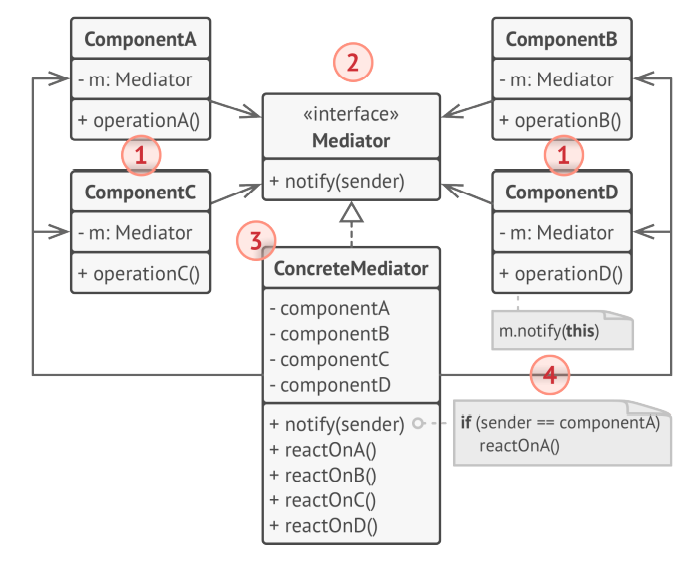
\includegraphics[scale=0.6]{image/behavioral/mediator.png}
\end{center}
\subsubsection{Ưu điểm và Nhược điểm}
Có các ưu điểm và nhược điểm sau:
Ưu điểm:
\begin{itemize}
    \item Đơn giản hóa cách giao tiếp giữa các đối tượng, Một Mediator sẽ thay thế mối quan hệ nhiều nhiều (many-to-many) giữa các component bằng quan hệ một-nhiều (one-to-many) giữa một mediator với các component.
    \item Quản lý tập trung, giúp làm rõ các component tương tác trong hệ thống như thế nào trong hệ thống.
    \item Giảm sự phụ thuộc giữa các đối tượng, làm cho hệ thống linh hoạt hơn và dễ dàng mở rộng.
    \item Tách biệt logic điều phối và logic của các đối tượng thành phần, làm cho mã dễ đọc và bảo trì hơn.
\end{itemize}
Nhược điểm:
\begin{itemize}
    \item Mediator có thể trở thành một điểm trung tâm phụ thuộc, làm giảm tính độc lập và sự tái sử dụng của các đối tượng thành phần.
\end{itemize}
\subsubsection{Code Example}
\begin{itemize}
    \item Có một interface Colleague và class User là subclass.
    \item Có một interface Mediator và class ChatRoom là subclass.
\end{itemize}
\begin{lstlisting}
#include <iostream>
#include <string>
#include <vector>

// Forward declaration
class Colleague;

// Mediator
class Mediator {
public:
    virtual void sendMessage(Colleague* sender, const std::string& message) = 0;
};

// Colleague (Abstract Base Class)
class Colleague {
protected:
    Mediator* mediator;

public:
    explicit Colleague(Mediator* mediator) : mediator(mediator) {}

    virtual void receiveMessage(const std::string& message) = 0;
    virtual void sendMessage(const std::string& message) = 0;
};

// Concrete Colleague
class User : public Colleague {
private:
    std::string name;

public:
    User(const std::string& name, Mediator* mediator) : name(name), Colleague(mediator) {}

    void receiveMessage(const std::string& message) override {
        std::cout << name << " received message: " << message << std::endl;
    }

    void sendMessage(const std::string& message) override {
        mediator->sendMessage(this, message);
    }
};

// Concrete Mediator
class ChatRoom : public Mediator {
private:
    std::vector<User*> users;

public:
    void addUser(User* user) {
        users.push_back(user);
    }

    void sendMessage(Colleague* sender, const std::string& message) override {
        for (auto user : users) {
            if (user != sender) {
                user->receiveMessage(message);
            }
        }
    }
};

int main() {
    ChatRoom chatRoom;

    User user1("Alice", &chatRoom);
    User user2("Bob", &chatRoom);
    User user3("Charlie", &chatRoom);

    chatRoom.addUser(&user1);
    chatRoom.addUser(&user2);
    chatRoom.addUser(&user3);

    user1.sendMessage("Hello, everyone!");
    user2.sendMessage("Hi, Alice!");

    return 0;
}

\end{lstlisting}
Ở hàm main, ta gọi 3 user cho vào chatRoom và thực hiện việc gửi tin nhắn.\\
\newline
\textbf{Kết quả:}
\begin{lstlisting}
Bob received message: Hello, everyone!
Charlie received message: Hello, everyone!
Alice received message: Hi, Alice!
Charlie received message: Hi, Alice!
\end{lstlisting}
\subsubsection{Các Pattern liên quan}
\begin{itemize}
    \item Chain of Responsibility truyền request lần lượt chứa các receiver tiềm năng cho đến khi có receiver thích hợp có thể giải quyết được. Command thì tạo ra các kết nối một chiều giữa các receiver và các sender.
    \item Mediator loại bỏ các kết nối trực tiếp giữa các receiver và các sender rồi bắt buộc chúng phải giao tiếp không trực tiếp thông qua đối tượng mediator.
    \item Observer cho phép các receiver chủ động trong việc subscribe và unsubscribe receiving requests.
    \item Facade thì định nghĩa một interface được đơn giản hóa đến các đối tượng của hệ thống con nhưng nó không tạo thêm các chức năng mới.
    \item Mediator thì sẽ trung gian hóa sự giao tiếp giữa các component trong hệ thống.
\end{itemize}